\section{原理}

\subsection{曲げ試験とは}
曲げ試験とは,単純な曲げ荷重を受ける材料の挙動を測定する試験である.具体的には試験片を2本の支持棒で支え,中央に荷重をかけて行う.セラミックスのような脆い脆性材料に対しては,引張試験が事実上困難であるという理由から多くの場合,曲げ試験を行い材料の機械特性,破壊特性を評価する.本実験においては,四点曲げ試験を行い材料の変形特性を評価した.

\subsection{原理}
四点曲げでは,はりの測定部にせん断応力はかからず,純粋な曲げモーメントがかかるため正確な弾性率を測定可能な手法である.
\begin{figure}[htbp]
    \centering %中央揃え
    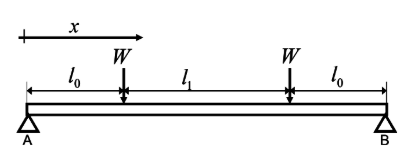
\includegraphics[width=100truemm,clip]{fig/fig_四点曲げ試験}
    \caption{Four-point bending.}
    \label{fig:fig_四点曲げ試験}
\end{figure}
図\ref{fig:fig_四点曲げ試験}のような四点曲げを想定したとき,それぞれ反力を$R_A$,$R_B$とすると,
\begin{equation}
    R_A + R_B = 2W
\end{equation}
点Bにおけるモーメントの釣り合いの条件から
\begin{equation}
    R_B(2l_0 + l_1) = Wl_0 + W(l_0 + l_1)
\end{equation}
したがって,
\begin{equation}
    R_A = R_B = W
\end{equation}
となり,はりにかかるせん断力$F$,曲げモーメント$M$は次のように示すことができる.

$0<x<l_0$
\begin{equation}
    F = R_A =W, M = R_Ax = Wx
\end{equation}

$l_0<x<l_0 + l_1$
\begin{equation}
    F = R_A - W = 0, M = R_Ax - W(x - l_0) = Wl_0
\end{equation}

$l_0 + l_1<x<2l_0 + l_1$
\begin{equation}
    F = R_A - W = -W, M = R_Ax - W(x - l_0) - W(x - l_0 - l_1) = W(2l_0 + l_1 - x)
\end{equation}

これより,曲げモーメント線図(Bending Moment Diagram:BMD),せん断力線図(Sharing Force Diagram:SFD)は図\ref{fig:BMD},\ref{fig:SFD}のように表すことができる.
\begin{figure}[htbp]
    \centering %中央揃え
    \includegraphics[width=100truemm,clip]{fig/fig_BMd}
    \caption{BMD.}
    \label{fig:BMD}
\end{figure}
\begin{figure}[htbp]
    \centering %中央揃え
    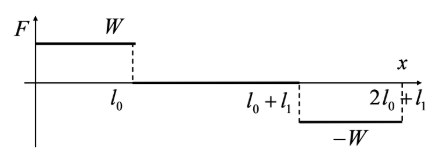
\includegraphics[width=100truemm,clip]{fig/fig_SFD}
    \caption{SFD.}
    \label{fig:SFD}
\end{figure}
このように四点曲げでは,測定部で曲げモーメントが一定であり,せん断応力がかからないことがわかる.

図\ref{fig:曲げモーメント断面}のようなはりの断面が長方形で一様な材料において,曲げによるはりに掛かる断面内の任意の位置の応力$\sigma (y)$は次のように表すことができる.
\begin{figure}[htbp]
    \centering %中央揃え
    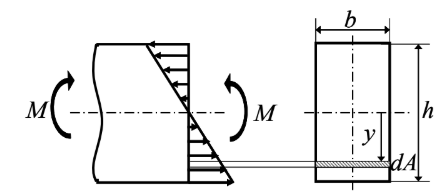
\includegraphics[width=100truemm,clip]{fig/fig_曲げ.png}
    \caption{Bending moment, bending stress applied to it, and beam cross section.}
    \label{fig:曲げモーメント断面}
\end{figure}
\begin{equation}
    \sigma (y) = \frac{M \cdot y}{I}
\end{equation}
$M$は曲げモーメント,$y$は中立軸からの距離,$I$は断面2次モーメントである.この応力は曲げによって生じるものであるから曲げ応力ともいわれる.曲げ応力は中立軸からはりの断面内で最も遠い距離で最大引張応力となり,次のように表すことができる.
\begin{equation}
   \sigma_{max} = \frac{M \cdot h}{2I}
\end{equation}
また,長方形の断面2次モーメントは次のように表せる.
\begin{equation}
    I = \int y^2dA = \frac{bh^3}{12}
\end{equation}

曲げモーメントおよびせん断応力を受けて変形したはりの軸線をたわみ曲線という.曲げモーメント$M$を受けて変形したはりの軸線の曲率半径を$\rho$とすると,その間には次式の関係がある.
\begin{equation}
    \frac{1}{\rho} = \frac{M}{EI}
\end{equation}
上式は$\rho$=一定の純曲げに対するもので,Eははりの材料の縦弾性係数である.また$EI$は曲げこわさという.曲げモーメントが針の長さに沿って変化する場合にも上の式はそれぞれの断面で成立するものと仮定すると,たわみ曲線の曲率半径もそれに応じて変化する.図\ref{fig:たわみ曲線}に示すように,はりの変形前の軸線のx軸,それに鉛直にy軸をとった場合,点xの垂直変位yをたわみといい,またたわみ曲線の点xにおける接線とx軸とのなす角$\theta$をたわみ角という.たわみ曲線は平面曲線でその曲率半径を$\rho$とすると次の式で表される.
\begin{figure}[htbp]
    \centering %中央揃え
    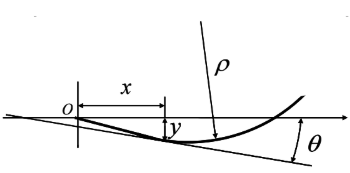
\includegraphics[width=100truemm,clip]{fig/fig_たわみ曲線.png}
    \caption{Deflection curve.}

    \label{fig:たわみ曲線}
\end{figure}
\begin{equation}
    \frac{1}{\rho} = \abs{\frac{d\theta}{ds}} = \abs{\frac{d\theta}{dx}} \frac{dx}{ds}, ds = \{(dx)^2 + (dy)^2\}^{1/2}, \mathrm{tan}\theta = \frac{dy}{dx}
\end{equation}
したがって
\begin{equation}
    \frac{1}{\rho} = \abs{\frac{d^2y}{dx^2}} /\{1 + (\frac{dy}{dx})^2\}^{3/2}
\end{equation}
曲げモーメントの符号は図\ref{fig:たわみ曲線}の座標軸をとると上に凹の曲率を生じる曲げモーメントを正としており,曲げモーメントが正の時は$\frac{d^2y}{dx^2} < 0$となる.また,たわみ曲線の傾斜の小さな変形を対象とすれば,$1 >> (\frac{dy}{dx})^2$であるから,
\begin{equation}
    \frac{d^2y}{dx^2} = -\frac{M}{EI}
\end{equation}
この式はたわみ曲線の微分方程式といい,たわみ曲線を求めるための基本となる式である.この式を解くとたわみ曲線は次のように表すことができる.
\begin{figure}[htbp]
    \centering %中央揃え
    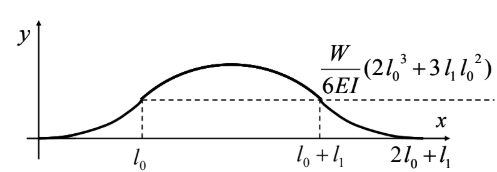
\includegraphics[width=100truemm,clip]{fig/fig_四点曲げたわみ曲線.png}
    \caption{Deflection curves for four-point bending.}
    \label{fig:曲げのたわみ曲線}
\end{figure}
\clearpage

